\documentclass{beamer}

%% Use package -----------------------------------------------------------------
\usepackage[T1]{fontenc}
\usepackage[utf8]{inputenc}
\usepackage{lmodern}
\usepackage{graphicx}
\usepackage[absolute,overlay]{textpos}
\usepackage{multicol}
\usepackage{listings}
\usepackage{svg}

%% Beamer customization---------------------------------------------------------

\usepackage{xcolor}
\usetheme{Warsaw}

%% Themes
% Outer themes
\useoutertheme{shadow}
% Rounded boxes and shadows
\useinnertheme[shadow=true]{rounded}
% Solid \item symbols
\useinnertheme{circles}

%% Custom colors
\definecolor{rltgreen}{rgb}{0,0.5,0}
\definecolor{pasteur}{RGB}{0,90,154}
\setbeamerfont{block title}{size={}}
\setbeamercolor{structure}{fg=pasteur}
\setbeamercolor{item}{fg=pasteur}

%Color of title
\setbeamertemplate{frametitle}
{
    \nointerlineskip
    \begin{beamercolorbox}[sep=0.3cm,ht=1.8em,wd=\paperwidth]{frametitle}
        \vbox{}\vskip-2ex%
        \strut\insertframetitle\strut
        \vskip-0.8ex%
    \end{beamercolorbox}
}
% Hide navigation symbols
\setbeamertemplate{navigation symbols}{}

%% Title block
\setbeamercolor*{title}{use=structure,fg=white,bg=pasteur}

\makeatletter

%% Top infolines
\setbeamertemplate{headline}{%
\leavevmode%
  \hbox{%
    \begin{beamercolorbox}[wd=\paperwidth,ht=2.5ex,dp=1.125ex]{palette quaternary}%
    \insertsectionnavigationhorizontal{\paperwidth}{}{\hskip0pt plus1filll}
    \end{beamercolorbox}%
  }
}

%% Define Snakemake ------------------------------------------------------------

\definecolor{eclipseBlue}{RGB}{42,0.0,255}
\definecolor{eclipseGreen}{RGB}{63,127,95}
\definecolor{eclipsePurple}{RGB}{127,0,85}

\lstset{language=Python}
\lstset{
    basicstyle=\tiny\ttfamily,
    morekeywords={rule, output, shell, params, run, configfile, temp},
    showstringspaces=false,
    commentstyle=\color{eclipseGreen}, % style of comments
    keywordstyle=\color{eclipsePurple}, % style of keywords
    stringstyle=\color{eclipseBlue}, % style of strings
}


%% Set up title ----------------------------------------------------------------

\title{A variant calling workflow using snakemake framework}
\author[D.Desvillechabrol \& T.Cokelaer]{Dimitri Desvillechabrol and Thomas Cokelaer}
\institute{Institut Pasteur}
\date{Sept 26th 2016, ENS Paris}



\AtBeginSection[]{
  \begin{frame}
  \vfill
  \centering
  \begin{beamercolorbox}[sep=8pt,center,shadow=true,rounded=true]{title}
    \usebeamerfont{title}\insertsectionhead\par%
  \end{beamercolorbox}
  \vfill
  \end{frame}
}

\begin{document}

%% Title slide -----------------------------------------------------------------

\begin{frame}[plain]
    \titlepage
    \begin{textblock*}{5cm}(4.5cm,0.3cm)
        
\includegraphics[scale=0.09]{images/Institut_Pasteur.png}
    \end{textblock*}
\end{frame}

%% Slides ----------------------------------------------------------------------

\section{Motivation}

\begin{frame}
 \frametitle{NGS at Biomics}
 
 Development driven by the Biomics Pole at Pasteur Institute, which involves
 many aspects of NGS including :
 
 \tiny
 \begin{block}{https://research.pasteur.fr/en/team/biomics/}
  \begin{itemize}
  \item De novo and targeted sequencing of viruses, prokaryotes and eukaryotes
  \item \textbf{Variant (SNP, indel, large rearrangements) detection}
  \item Human and Mouse SNP detection by array
  \item Transcriptional analysis (RNA-Seq) for both prokaryotes and eukaryotes
  \item 16S and deep-sequencing metagenomic studies (mouse, human, and other environments)
  \item Bottom-up whole proteomic analysis and quantification
  \item Analysis of a wide range of post-translational modifications
  \item Determination of the dynamics of protein complexes.
  \item Epigenetics (methylation studies)
  \item Projects involving two or more techniques (i.e. proteogenomics, single-cell DNA/RNA analysis)
  \end{itemize}
 \end{block}
 \small 
\end{frame}



\section{Sequana project}

\begin{frame}
    \frametitle{What is Sequana ?}
    \begin{block}{1. A Python library}
       \tiny
    \begin{itemize}
        \item Pandas for data mining, matplotlib for visualisation and the Python ecosystem (e.g., scipy)
        \item Tools to simplify the interface with external dependencies (e.g., snpEff, kraken)
        \item More advanced NGS data structures (e.g., BAM reader with plotting functionalities)
    \end{itemize} 
    \end{block}
    \pause
    
    \begin{block}{2. A framework to store/design pipelines}
    \tiny
    \begin{itemize}
        \item Using Snakemake as a common language to design new pipelines
        \item Provide reusable snakemake rules and modules
    \end{itemize} 
     \end{block}
  \pause
  
    \begin{block}{3. A set of HTML reports}
    \tiny
    \begin{itemize}
	\item We use JINJA templating to re-use HTML templates
    \end{itemize} 
    \end{block}
  \pause  
    \begin{block}{4. A suite of standalone applications}
    \tiny
    \begin{itemize}
	\item sequana (create pipeline and config file locally)
	\item sequana\_coverage
	\item sequana\_mapping
	\item \dots
    \end{itemize} 
    \end{block}
\end{frame}

\begin{frame}[fragile]{What is Snakemake ?}
    \begin{columns}
    \begin{column}{0.6\textwidth}
    \begin{itemize}
        \item It is a workflow manager based on python
        \begin{itemize}
            \item Parallelization
            \item Suspend/Resume
            \item Simplify the workflow's conceptions
            \item Decompose workflow into rules
        \end{itemize}
    \end{itemize}
    \begin{block}{Rule example}
    \begin{lstlisting}
rule bedtools_genomecov:
    input:
        __bedtools_genomecov__input
    output:
        __bedtools_genomecov__output
    params:
        options = config["bedtools"]["options"]
    shell:
        """
        bedtools genomecov {params.options} \
        -ibam {input} > {output}
        """ 
    \end{lstlisting}
    \end{block}
    \end{column}
    \begin{column}{0.4\textwidth}
        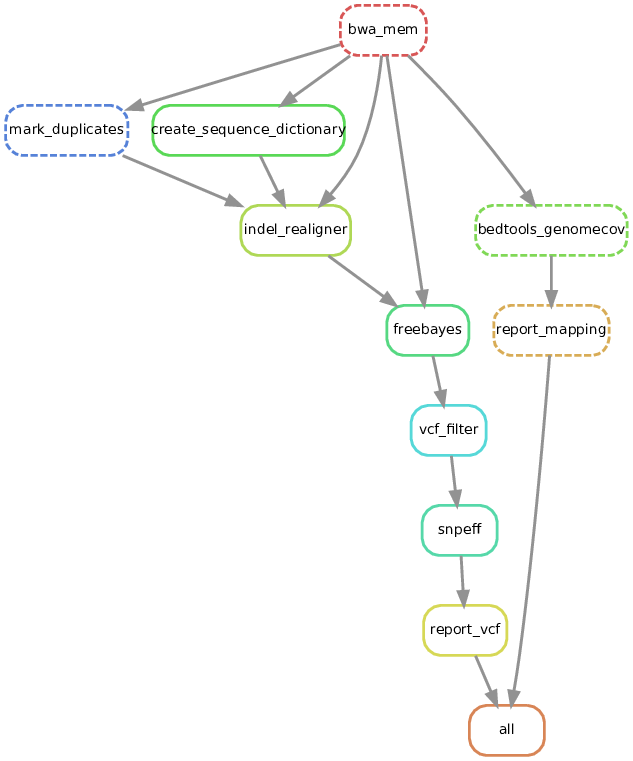
\includegraphics[scale=0.21]{images/variant_calling_dag}
    \end{column}
    \end{columns}
\end{frame}

\section{Variant calling}

\begin{frame}{Variant calling overview}
    \begin{itemize}
        \item Detect SNPs/INDELs of a sequenced sample against a reference genome 
            or assembled set of contigs
        \begin{itemize}
            \item Align reads on a reference
            \item Mark duplicates and realign reads around INDELs
            \item Run a variant caller to detect SNPs and INDELs
            \item Interpret results
        \end{itemize}
    \end{itemize}
\end{frame}

\begin{frame}{The variant calling pipeline}
    \center
    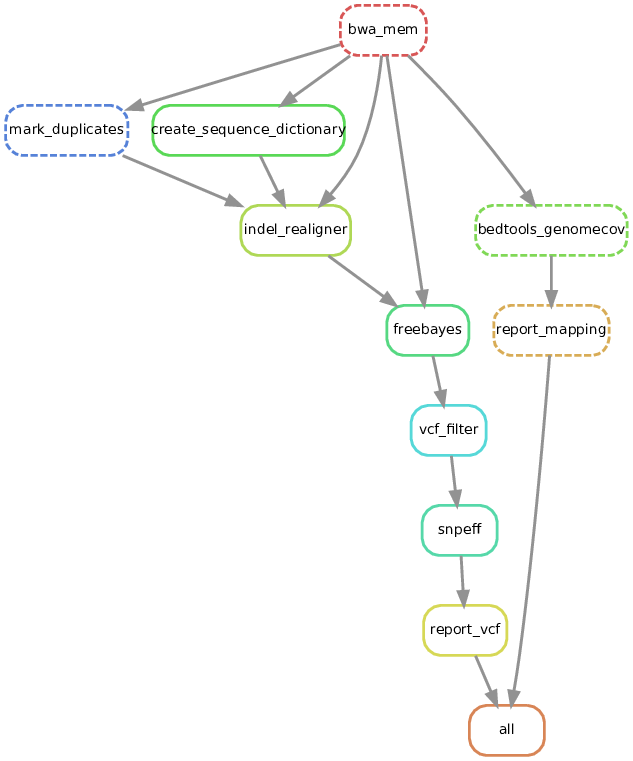
\includegraphics[scale=0.28]{images/variant_calling_dag}
\end{frame}

\begin{frame}{Mapping analysis}
    \begin{itemize}
        \item Check the quality of mapping
    \end{itemize}
    \center
    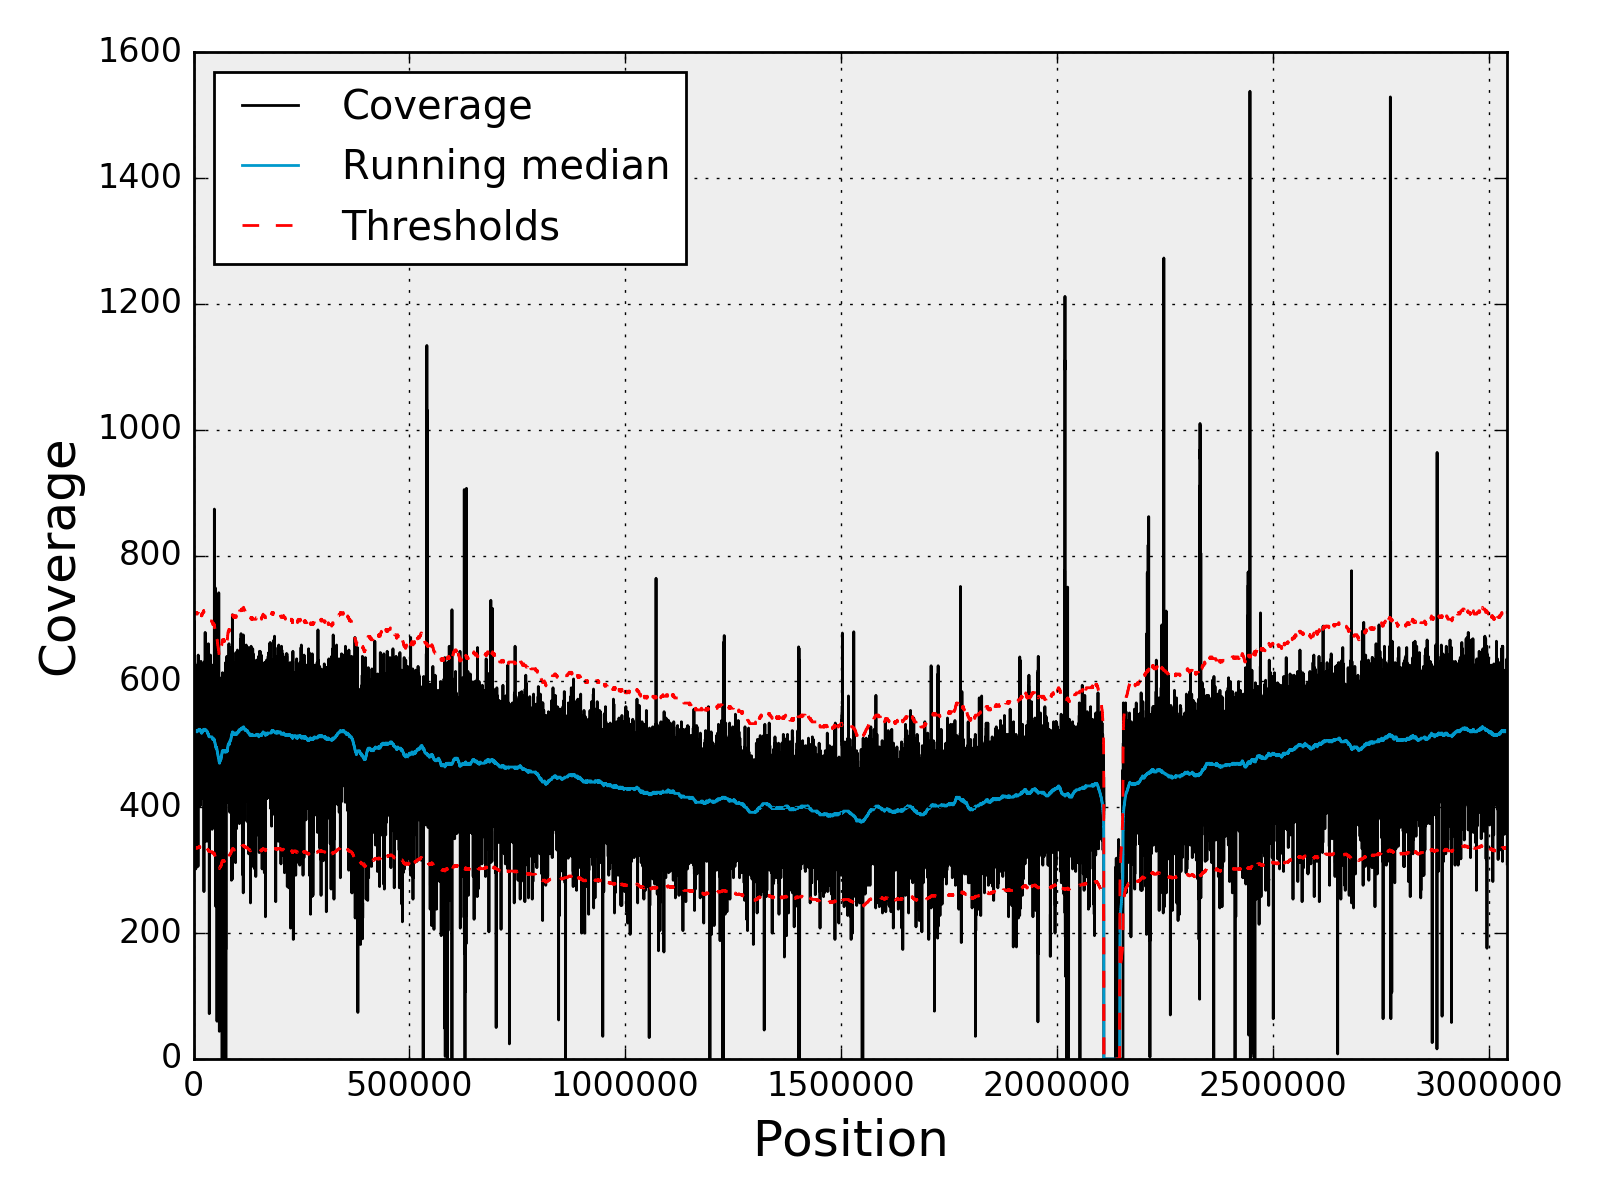
\includegraphics[scale=0.4]{images/running_median}
\end{frame}

\begin{frame}{High and low coverage regions detection}
    \begin{textblock*}{10cm}(0.2cm,2cm)
        \begin{itemize}
            \item High coverage regions
        \end{itemize}
        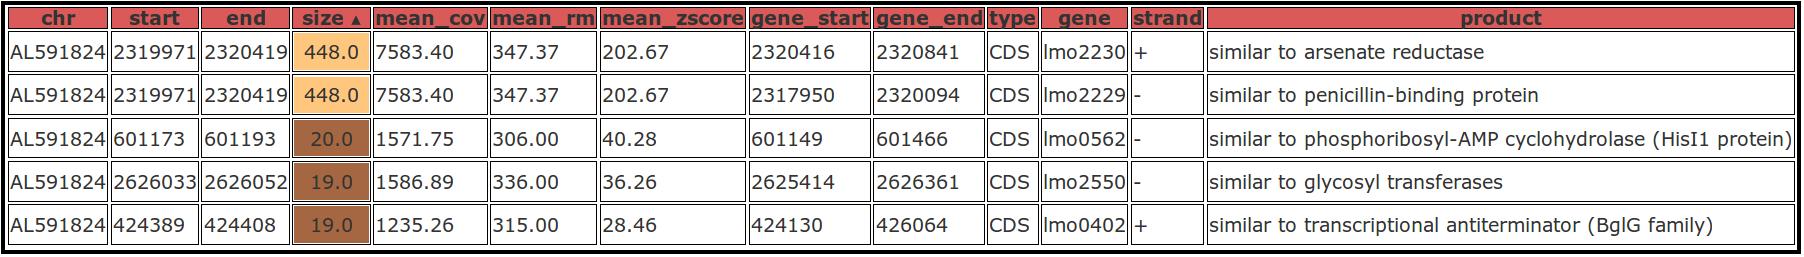
\includegraphics[scale=0.195]{images/high_roi}
    \end{textblock*}
    \begin{textblock*}{10cm}(0.2cm, 5cm)
        \begin{itemize}
            \item Low coverage regions
        \end{itemize}
        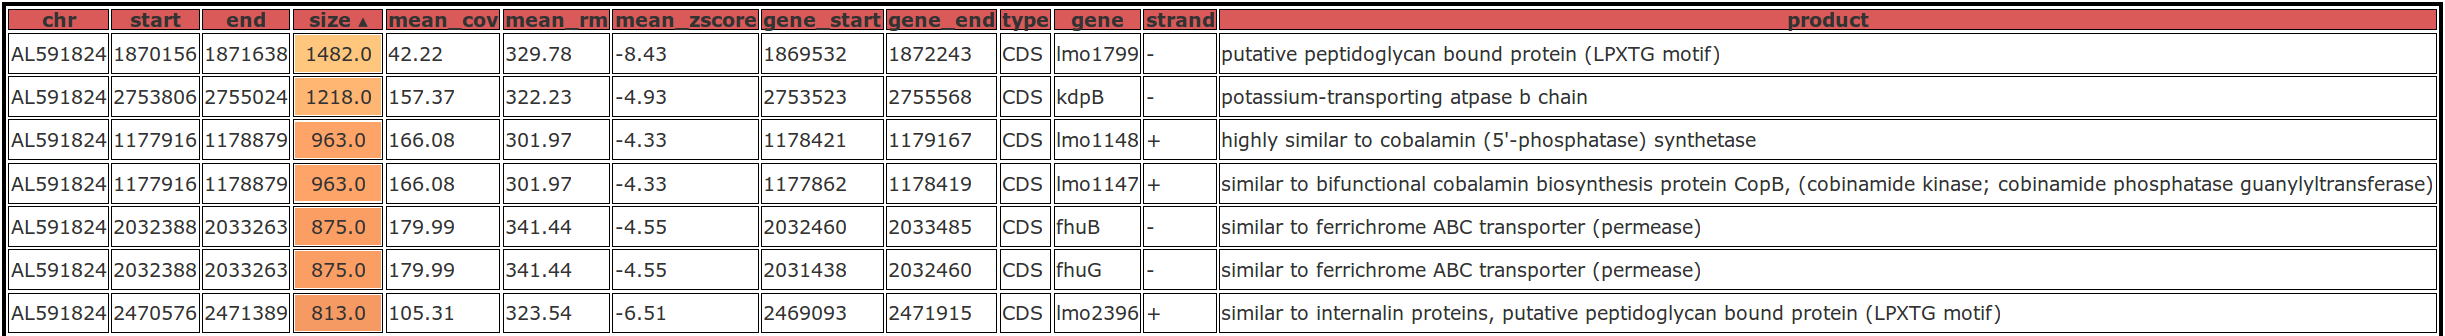
\includegraphics[scale=0.145]{images/low_roi}
    \end{textblock*}
\end{frame}

\begin{frame}{Javascript interface}
    \begin{itemize}
        \item Implemented a Javascript and HTML5 visualisation toolbox with zoomable plot
    \end{itemize}
    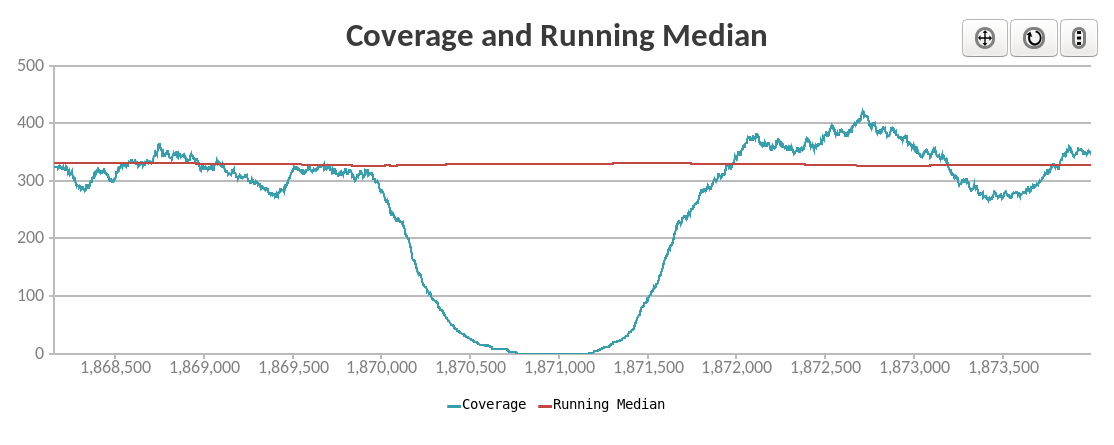
\includegraphics[scale=0.28]{images/js_graphic}
\end{frame}

\begin{frame}{Variant calling}
    \begin{itemize}
        \item Variants are detected with Freebayes
        \item The python module PyVCF is used to filter variants
    \end{itemize}
    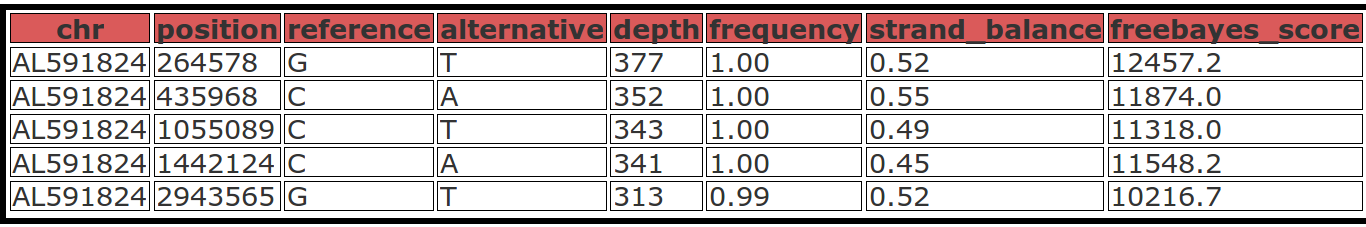
\includegraphics[scale=0.23]{images/freebayes}
    \begin{itemize}
        \item Variants are annotated with snpEff
    \end{itemize}
    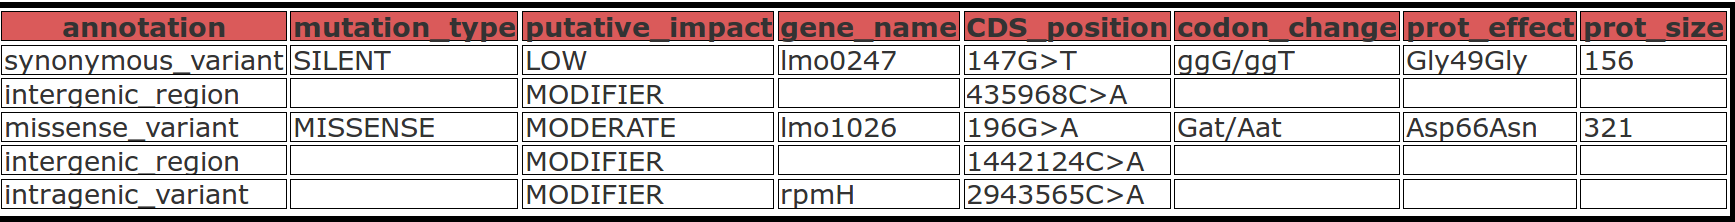
\includegraphics[scale=0.18]{images/snpeff}
\end{frame}

\section{Usage}

\begin{frame}[fragile]{Set up the pipeline}
    \begin{itemize}
        \item One command line to initiate the pipeline
    \end{itemize}
    \begin{lstlisting}
sequana --pipeline variant_calling --file1 R1.fastq.gz --file2 R2.fastq.gz \
    --reference sequence.fasta --project project_1
    \end{lstlisting}
    \begin{itemize}
        \item The sequana executable creates a directory with the project name
        \item The directory contains all the necessary files (config, snakefile,~\dots)
    \end{itemize}
\end{frame}

\begin{frame}[fragile]{Run the pipeline}
    \begin{itemize}
        \item You just need to launch snakemake
    \end{itemize}
    \begin{lstlisting}
snakemake -s variant_calling.rules --cluster "qsub -q queue -cwd -V" -j 6
    \end{lstlisting}
    \begin{itemize}
        \item Snakemake is compatible with all job schedulers
    \end{itemize}
\end{frame}

\section{Continuous integration}

\begin{frame}
 \frametitle{Versioning}
Sequana is available on GitHub (github.com/sequana/sequana). Started in Feb. 2016. 
About 1000 commits. 260 issues created (15 currently open) \\
\begin{center}
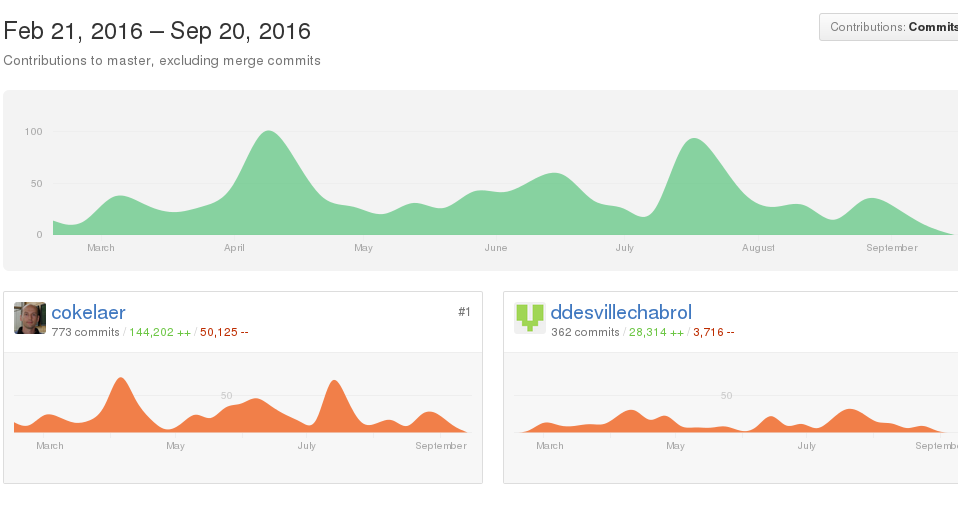
\includegraphics[scale=0.2]{images/commits}
\end{center}

\end{frame}



\begin{frame}
    \frametitle{Test suite}
    \begin{block}{}
    Continuous Integration on Travis with 60 tests with 60\% coverage
    \end{block}
    
    
    %\begin{textblock*}{7cm}(.5cm,3.5cm)
        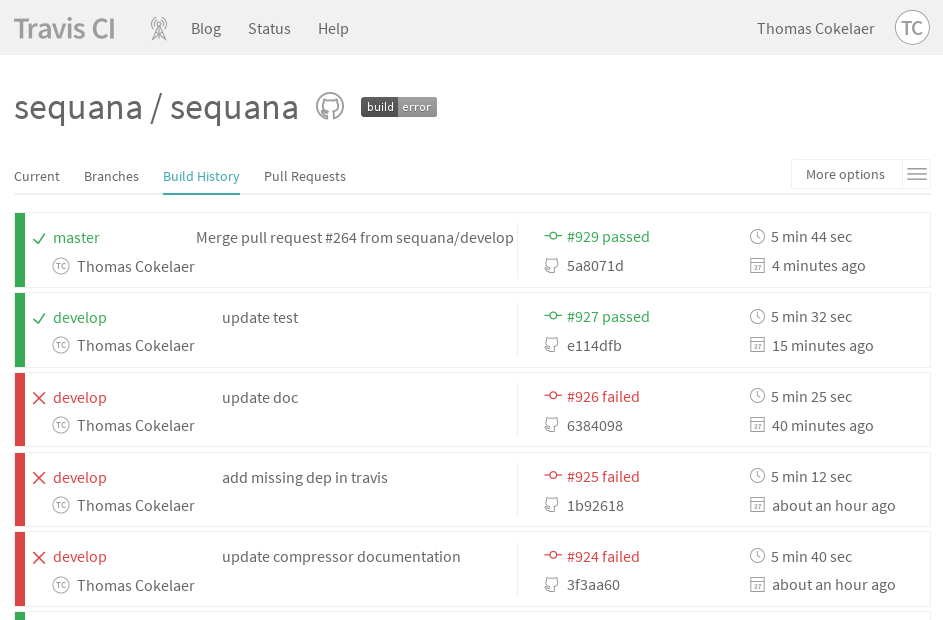
\includegraphics[scale=0.35]{images/travis}
    %\end{textblock*}
\end{frame}


\begin{frame}
    \frametitle{Documentation}
    Fully documented and available on sequana.readthedocs.org~.
    Uses Sphinx (RST syntax) to document the source code and provides user guide.
    Updated automatically at each commits.
\begin{center}
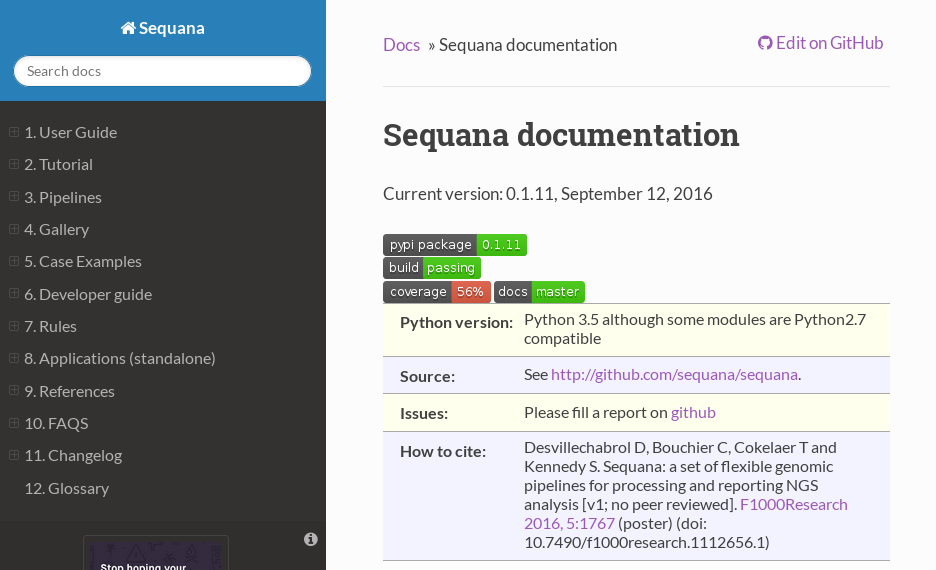
\includegraphics[scale=0.3]{images/rtd}
\end{center}
\end{frame}




\section{Summary and Future Directions}
\begin{frame}

\begin{block}{Pipelines to come}
\begin{itemize}
 \item PacBio was acquired recently. Next pipeline will include
 a long-read analysis. Creation of snakefile pipelines to compare performance 
 of different long-read software.
\end{itemize}
\end{block}

\begin{block}{Future developments}
 \begin{itemize}
  \item Simple GUI to ease the creation of the analysis pipelines.
  \item Docker images to help integration in different platforms.
 \end{itemize}
\end{block}
 \end{frame}

\end{document}


